\section{Resultados} \label{sec:resultados}

\subsection{Efecto disciplinador}

La Figura \ref{fig:es_principal} presenta el estudio de eventos de \eqref{eq:es} para los cuatro combustibles, estimado por efectos fijos bidireccionales (TWFE) y con el estimador de \textcite{SUNABRAHAM2021}. Los coeficientes son cambios porcentuales del precio de las incumbentes respecto del semestre previo a la entrada.

\begin{figure}[htbp]
    \centering
    \caption{Efecto de la entrada sobre el precio de las incumbentes, ventana 2012 a 2026} \label{fig:es_principal}
    
\includegraphics{output/graficos/sunab_2012_2026.pdf}
    \caption*{\footnotesize Fuente: Precios históricos de bencinaenlinea.cl. Panel mensual de estaciones, log del precio $\times$ 100. Tratadas son estación con una entrada competidora a 2 km o menos, controles son estación sin entradas a menos de 5 km. El eje horizontal está en semestres, bins de seis meses desde la entrada, con extremos agrupados ($\leq -4$ y $\geq 4$) y referencia en $-1$. Efectos fijos de estación, mes, región $\times$ año y marca $\times$ año. Estimadores Sun y Abraham con cohortes mensuales y las nunca tratadas como referencia. Intervalos al 95\% con errores estándar agrupados por comuna. Tratadas y controles, 501 y 373 en gasolina 93, 503 y 375 en gasolina 95, 471 y 313 en gasolina 97, 506 y 383 en diésel.}
\end{figure}

La entrada reduce el precio de las incumbentes en los cuatro combustibles. En la gasolina 93 el precio cae 0,30\% en el semestre de la entrada y se estabiliza en torno a 0,40\% desde el segundo semestre, sin revertirse. En la gasolina 95 la caída es de 0,38\% en el primer semestre y de 0,48\% en el segundo, y luego se mantiene entre 0,31\% y 0,41\%, significativa en todos los bins. En la gasolina 97 el efecto es de 0,33\% y 0,40\% en el primer año y deja de ser distinguible de cero desde el tercer semestre. El diésel tiene el efecto más grande y más persistente, 0,46\% en el primer semestre, que crece hasta 0,61\% desde el cuarto semestre. Como el costo mayorista es el mismo para todas las estaciones en un mes y lo absorbe el efecto fijo de mes, la caída de precio de las incumbentes es una caída de su margen. Los resultados apoyan la Hipótesis 1.

Los coeficientes previos a la entrada apoyan el supuesto de tendencias paralelas. Con TWFE ningún bin previo es distinto de cero al 10\% en ningún combustible, todos son menores a 0,07\% en valor absoluto y no muestran una tendencia antes de la entrada. Con \textcite{SUNABRAHAM2021} el bin $-2$ es positivo y significativo al 10\% en las gasolinas 93 y 95 y en el diésel, con magnitudes de 0,07\% a 0,08\%, menos de un cuarto del efecto del primer semestre.

Los dos estimadores entregan el mismo resultado. Las estimaciones de \textcite{SUNABRAHAM2021} están dentro de los intervalos de TWFE en todos los bins y combustibles, y son levemente más negativas en el bin $\geq 4$ de las gasolinas 93 y 95. La heterogeneidad entre cohortes no cambia de forma relevante la estimación TWFE.

La Tabla \ref{tab:es_p93} muestra cómo cambia la estimación de la gasolina 93 al agregar efectos fijos. Sin efectos fijos (columna 1) los coeficientes no tienen sentido económico, porque la variación del precio en el tiempo domina la comparación. Al incluir el efecto fijo de mes (columna 2) los bins previos pasan a ser cero y el efecto del primer semestre es de 0,37\%. Agregar los efectos fijos de estación, región $\times$ año y marca $\times$ año (columnas 3 a 5) reduce el efecto del primer semestre de 0,37\% a 0,30\%, mantiene su significancia al 1\% y deja los bins previos en cero. En el bin $\geq 4$ el efecto pasa de 0,79\% a 0,42\%. Los factores fijos de cada estación y los shocks anuales de cada región y de cada marca explican parte de la diferencia de largo plazo, pero no generan el efecto de la entrada, lo que respalda el supuesto de que el momento de la entrada es exógeno a las incumbentes. Las Tablas \ref{tab:es_p97} y \ref{tab:es_pdi} muestran el mismo patrón para la gasolina 97 y el diésel. En la gasolina 97 el bin $-3$ es significativo al 10\% en las columnas 2 y 3 y deja de serlo al incluir el efecto fijo de región $\times$ año. En el diésel el bin $-2$ es significativo al 10\% en la columna 2 y deja de serlo al incluir el efecto fijo de estación.

\begin{table}[htbp]
    \centering
    \caption{Estudio de eventos por especificación de efectos fijos, gasolina 93} \label{tab:es_p93}
    
\begingroup
\centering
\begin{tabular}{lccccc}
   \toprule
                        & (1)             & (2)            & (3)            & (4)            & (5)\\  
   \midrule 
   $\leq -4$            & -4.293$^{***}$  & 0.096          & 0.022          & -0.021         & -0.002\\   
                        & (1.308)         & (0.193)        & (0.148)        & (0.093)        & (0.086)\\   
   $-3$                 & -0.779          & 0.017          & 0.002          & -0.022         & -0.017\\   
                        & (1.108)         & (0.087)        & (0.082)        & (0.061)        & (0.062)\\   
   $-2$                 & -0.018          & 0.034          & 0.042          & 0.060          & 0.058\\   
                        & (0.814)         & (0.076)        & (0.070)        & (0.067)        & (0.067)\\   
   $0$                  & -1.146          & -0.374$^{***}$ & -0.357$^{***}$ & -0.316$^{***}$ & -0.296$^{***}$\\   
                        & (0.853)         & (0.106)        & (0.101)        & (0.096)        & (0.094)\\   
   $1$                  & -1.710          & -0.525$^{***}$ & -0.478$^{***}$ & -0.429$^{***}$ & -0.401$^{***}$\\   
                        & (1.152)         & (0.114)        & (0.100)        & (0.106)        & (0.107)\\   
   $2$                  & -2.152          & -0.562$^{***}$ & -0.493$^{***}$ & -0.430$^{***}$ & -0.400$^{***}$\\   
                        & (1.568)         & (0.145)        & (0.113)        & (0.119)        & (0.118)\\   
   $3$                  & -0.630          & -0.654$^{***}$ & -0.557$^{***}$ & -0.423$^{***}$ & -0.399$^{***}$\\   
                        & (1.653)         & (0.191)        & (0.156)        & (0.142)        & (0.138)\\   
   $\geq 4$             & 22.746$^{***}$  & -0.792$^{**}$  & -0.721$^{***}$ & -0.446$^{***}$ & -0.423$^{***}$\\   
                        & (1.741)         & (0.306)        & (0.173)        & (0.140)        & (0.135)\\   
   Tratada              & -10.704$^{***}$ & -1.598$^{***}$ &                &                &   \\   
                        & (1.739)         & (0.326)        &                &                &   \\   
   Tratadas             & 501             & 501            & 501            & 501            & 501\\  
   Controles            & 377             & 377            & 373            & 373            & 373\\  
    \\
   Observaciones        & 124,438         & 124,438        & 124,434        & 124,434        & 124,427\\  
    \\
   Mes                  & No              & Sí             & Sí             & Sí             & Sí\\  
   Estación             & No              & No             & Sí             & Sí             & Sí\\  
   Región $\times$ año  & No              & No             & No             & Sí             & Sí\\  
   Marca $\times$ año   & No              & No             & No             & No             & Sí\\  
   \bottomrule
\end{tabular}
\par\endgroup



    \caption*{\footnotesize Fuente: Precios históricos de bencinaenlinea.cl. Panel mensual 2012 a 2026, log del precio $\times$ 100. Errores estándar agrupados por comuna entre paréntesis. * p$<$0,10 ** p$<$0,05 *** p$<$0,01. Bins de seis meses desde la entrada, referencia en $-1$. Tratadas son estación con una entrada competidora a 2 km o menos, controles son estaciones sin entradas a menos de 5 km. Sin efecto fijo de estación (columnas 1 y 2) se controla por el indicador de tratada. Tratadas y controles son estaciones que usa cada modelo.}
\end{table}

\subsection{Atenuación espacial}

La Figura \ref{fig:atenuacion} presenta el efecto de la entrada por anillo de distancia entre la incumbente y la entrante, estimado con \eqref{eq:es_est}. Cada coeficiente es el efecto promedio de los primeros seis meses tras la entrada.

\begin{figure}[htbp]
    \centering
    \caption{Efecto de la entrada sobre el precio de las incumbentes por distancia a la entrante} \label{fig:atenuacion}
    
\includegraphics{output/graficos/atenuacion_distancia.pdf}
    \caption*{\footnotesize Fuente: Precios históricos de bencinaenlinea.cl. Panel mensual 2012 a 2026, log del precio $\times$ 100. Efecto estático por anillo de distancia a la primera entrada competidora a 5 km o menos. Las tratadas aportan los seis meses antes y los seis meses después de la entrada, los controles, estaciones sin entradas a menos de 5 km, aportan todos sus meses. Efectos fijos de estación, mes, región $\times$ año y marca $\times$ año. Intervalos al 95\% con errores estándar agrupados por comuna. Entre 89 y 125 tratadas por anillo y entre 313 y 383 controles según el combustible.}
\end{figure}

El efecto decrece con la distancia y desaparece a partir de los 3 kilómetros. Entre 0 y 1 kilómetro el precio de las incumbentes cae entre 0,57\% (gasolina 97) y 0,74\% (gasolina 95). Entre 1 y 2 kilómetros la caída es de 0,37\% a 0,47\%, alrededor de dos tercios del efecto del primer anillo. Entre 2 y 3 kilómetros el efecto sigue siendo significativo en los cuatro combustibles, con caídas de 0,28\% (diésel) a 0,49\% (gasolina 97). Entre 3 y 4 kilómetros y entre 4 y 5 kilómetros ningún coeficiente es distinto de cero. En las gasolinas 93 y 95 el coeficiente de 4 a 5 kilómetros es cercano a cero, de 0,05\% y 0,11\%. En la gasolina 97 y el diésel los coeficientes de 3 a 5 kilómetros están entre 0,18\% y 0,32\%, pero con intervalos amplios que incluyen el cero. Entre los anillos con efecto significativo, la gasolina 97 es la única en que el efecto no decrece de forma monótona, ya que el de 2 a 3 kilómetros es mayor que el de 1 a 2. Los resultados apoyan la Hipótesis 2.

El umbral tiene relevancia para la definición del mercado relevante geográfico. La \textcite{FNE2021informe} señala que en general la presión competitiva relevante se ha considerado en radios de 3 o 5 kilómetros. En ese caso concluye que el mercado relevante no debiera superar los 3 kilómetros. Los resultados respaldan el radio de 3 kilómetros, dentro de él la entrada reduce el precio de las incumbentes y fuera de él el efecto no es distinguible de cero. Un radio de 5 kilómetros incluiría estaciones sobre las que no se detecta presión competitiva. A la vez, un radio menor a 3 kilómetros dejaría fuera estaciones entre 2 y 3 kilómetros que sí responden a la entrada.

Adicionalmente, se estimó el efecto por separado para las incumbentes ubicadas a 100 metros o menos de la red vial primaria (autopistas y rutas nacionales). La Tabla \ref{tab:het_autopista} y la Figura \ref{fig:het_autopista} reportan los resultados. En las incumbentes que no están junto a una autopista la entrada reduce el precio entre 0,37\% (gasolina 97) y 0,66\% (diésel). En las incumbentes de autopista el efecto no es negativo en ningún combustible: es cercano a cero y no significativo en las gasolinas 93 y 95 y en el diésel, y positivo y significativo al 5\% en la gasolina 97. La diferencia entre ambos grupos es significativa al 1\% en las tres gasolinas y al 10\% en el diésel. La comparación no aísla un efecto causal de la autopista, pero es consistente con que para una estación de autopista una parte importante de la demanda va de paso, por lo que su mercado relevante es el corredor vial y no el radio en torno a ella. Un radio fijo de 3 kilómetros es adecuado para estaciones urbanas, pero no para estaciones de autopista, cuyo mercado relevante debiera definirse a lo largo de la ruta.

\subsection{Asimetría distributiva}

La Tabla \ref{tab:mercado} presenta el efecto de la entrada sobre el percentil 90, la mediana y el percentil 10 de los precios del mercado local, estimado con \textcite{SUNABRAHAM2021}. El percentil 90 representa a las estaciones caras del mercado, el percentil 10 a las baratas y la mediana al centro. El mercado incluye a la estación que abre. La Figura \ref{fig:mercado} presenta el estudio de eventos de las mismas series.



\begin{figure}[htbp]
    \centering
    \caption{Estudio de eventos sobre los precios del mercado local} \label{fig:mercado}
    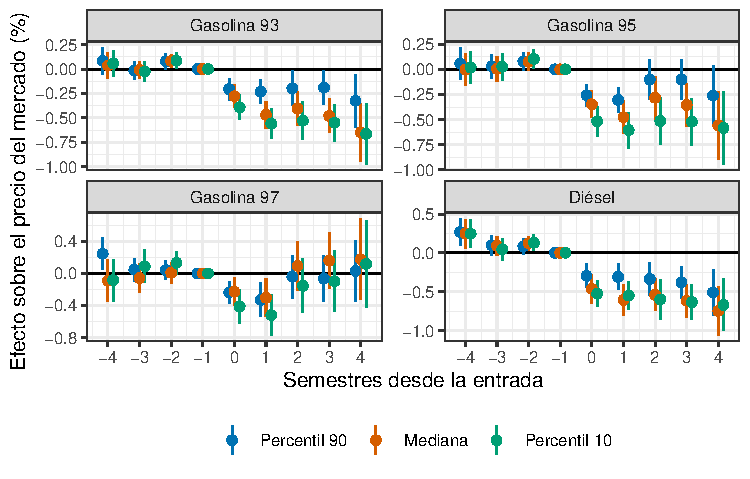
\includegraphics{output/graficos/mercado.pdf}
    \caption*{\footnotesize Fuente: Precios históricos de bencinaenlinea.cl. Estudio de eventos con estimadores Sun y Abraham con cohortes mensuales sobre el log del percentil 90, la mediana y el percentil 10 de los precios del mercado $\times$ 100. Eje horizontal en semestres, bins de seis meses desde la entrada, extremos agrupados, referencia en $-1$. Intervalos al 95\% con errores estándar agrupados por comuna. Mercados, muestra y efectos fijos como en la Tabla \ref{tab:mercado}.}
\end{figure}

La entrada reduce más los precios bajos que los altos. En la gasolina 93 el percentil 10 cae 0,62\%, la mediana 0,58\% y el percentil 90 0,29\%. En la gasolina 95 las caídas son de 0,57\%, 0,50\% y 0,24\%, esta última significativa solo al 10\%. En el diésel son de 0,64\%, 0,69\% y 0,46\%. En los tres combustibles la parte baja del mercado cae más que la alta, con una brecha de 0,33 puntos en las gasolinas 93 y 95 y de 0,19 puntos en el diésel, por lo que la entrada aumenta la dispersión de precios del mercado. En la gasolina 97 ningún efecto es distinto de cero.

La Figura \ref{fig:mercado} muestra la dinámica. En la gasolina 93 los bins previos son cercanos a cero, salvo el bin $-2$, levemente positivo en los tres cuantiles (0,08\%). Después de la entrada el percentil 90 cae en torno a 0,2\% y se mantiene, mientras que la mediana y el percentil 10 se profundizan hasta 0,65\% en el bin $\geq 4$. En la gasolina 95 el percentil 10 cae 0,52\% en el primer semestre y 0,60\% en el segundo, y el percentil 90 cae 0,26\% y 0,30\% en el primer año y deja de ser distinguible de cero desde el tercer semestre. En la gasolina 97 los precios del mercado caen solo en los dos primeros semestres, más en el percentil 10 (0,41\% y 0,52\%), y el percentil 90 tiene un bin $-4$ positivo y significativo. En el diésel los bins $-4$ y $-2$ son positivos y significativos, de 0,25\% y 0,12\%, por lo que los precios del mercado ya venían cayendo antes de la entrada. Los resultados apoyan la Hipótesis 3 en las gasolinas 93 y 95, en el diésel con la salvedad de la tendencia previa, y no en la gasolina 97.

La Figura \ref{fig:distribucion_beta} presenta el perfil de $\beta(c)$ de la regresión de distribución para los 41 umbrales, y la Figura \ref{fig:distribucion_acumulada} la distribución acumulada observada de las tratadas después de la entrada junto a su contrafactual.

\begin{figure}[htbp]
    \centering
    \caption{Desplazamiento de la distribución de precios por efecto de la entrada} \label{fig:distribucion_beta}
    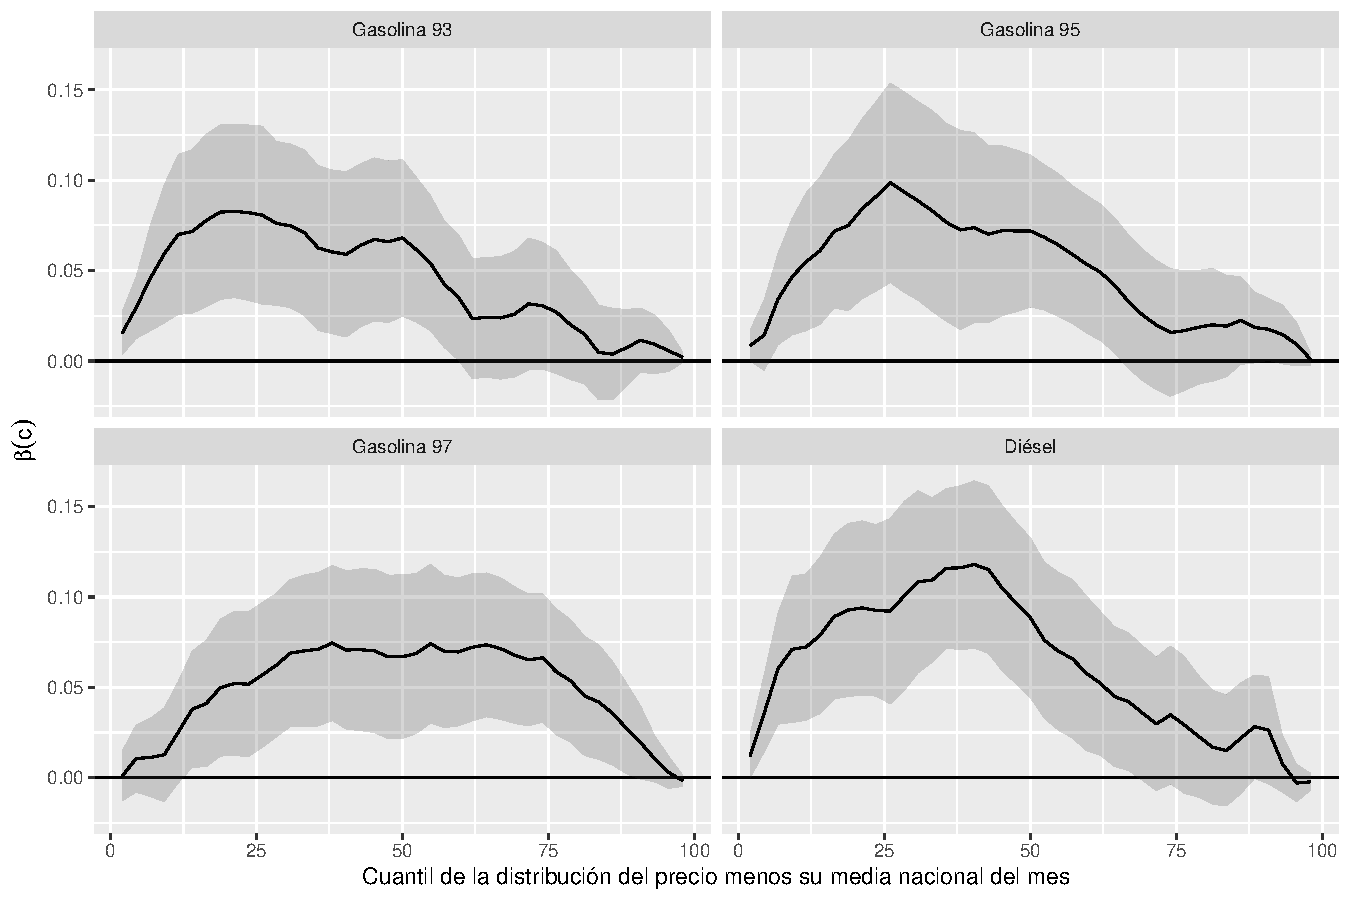
\includegraphics{output/graficos/distribucion_beta.pdf}
    \caption*{\footnotesize Fuente: Precios históricos de bencinaenlinea.cl. Panel mensual 2012 a 2026. Cada punto es una regresión de $\mathbf{1}[\tilde{p}_{it} \leq c]$ sobre el indicador de entrada, con $\tilde{p}_{it}$ el precio menos su media nacional del mes y $c$ el umbral correspondiente al cuantil del eje horizontal. $\beta(c) > 0$ indica más masa bajo $c$, es decir, precios más bajos. Efectos fijos de estación, mes, región $\times$ año y marca $\times$ año. Bandas al 95\% con errores estándar agrupados por comuna. Control: estaciones sin entradas a menos de 5 km.}
\end{figure}

\begin{figure}[htbp]
    \centering
    \caption{Distribución de precios con y sin entrada} \label{fig:distribucion_acumulada}
    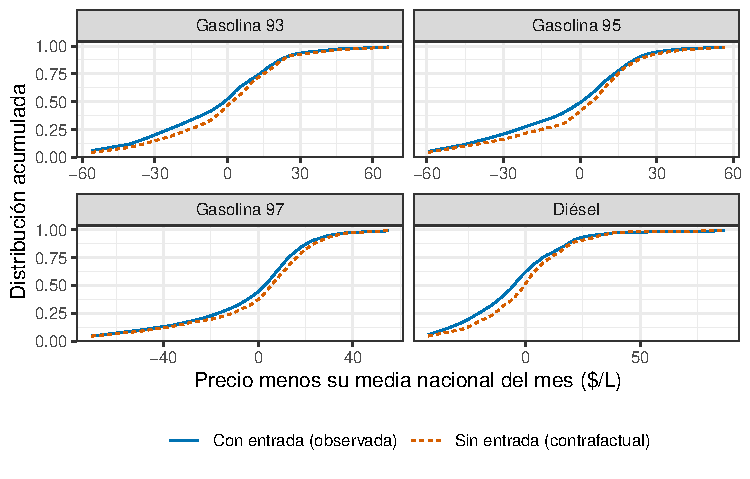
\includegraphics{output/graficos/distribucion_acumulada.pdf}
    \caption*{\footnotesize Fuente: Precios históricos de bencinaenlinea.cl. Distribución acumulada del precio menos su media nacional del mes para las tratadas después de la entrada (observada) y la que habrían tenido sin la entrada (observada menos $\beta(c)$), sobre 41 umbrales entre los cuantiles 2 y 98. Misma muestra y regresiones que la Figura \ref{fig:distribucion_beta}.}
\end{figure}

La entrada desplaza la distribución de precios hacia valores menores y el desplazamiento se concentra en la mitad baja. En la gasolina 93 la entrada aumenta en 5,9 puntos porcentuales la proporción de precios bajo el cuantil 10, en 8,1 bajo el cuantil 25 y en 6,8 bajo la mediana, y el efecto cae a 3,1 puntos en el cuantil 75 y a 1,1 puntos, no significativo, en el cuantil 90. La gasolina 95 tiene el mismo patrón, con un máximo de 9,9 puntos en el cuantil 25. En el diésel el máximo es de 11,8 puntos en torno al cuantil 40 y el efecto cae a 2,6 puntos en el cuantil 90. La gasolina 97 es la excepción: el efecto es nulo en el cuantil 10 y se mantiene entre 5,7 y 6,7 puntos desde el cuantil 25 hasta el 75, por lo que el desplazamiento se ubica en el centro de la distribución y no en la cola baja.
